%%%%%% CMB-S4 Simulations and Data Analysis Chapter, Sky Modeling Section  %%%%%%%%%%%%%%%%

\section{Sky Modeling}

Key challenges: 
\begin{itemize} 
\item reliability of models based on noisy, bandpassed, beam-convolved observations, including Planck
\item self-consistency of CMB secondaries and extra-Galactic foregrounds
\item usability/software engineering
\end{itemize} 

\begin{figure}[htbp]
\centering
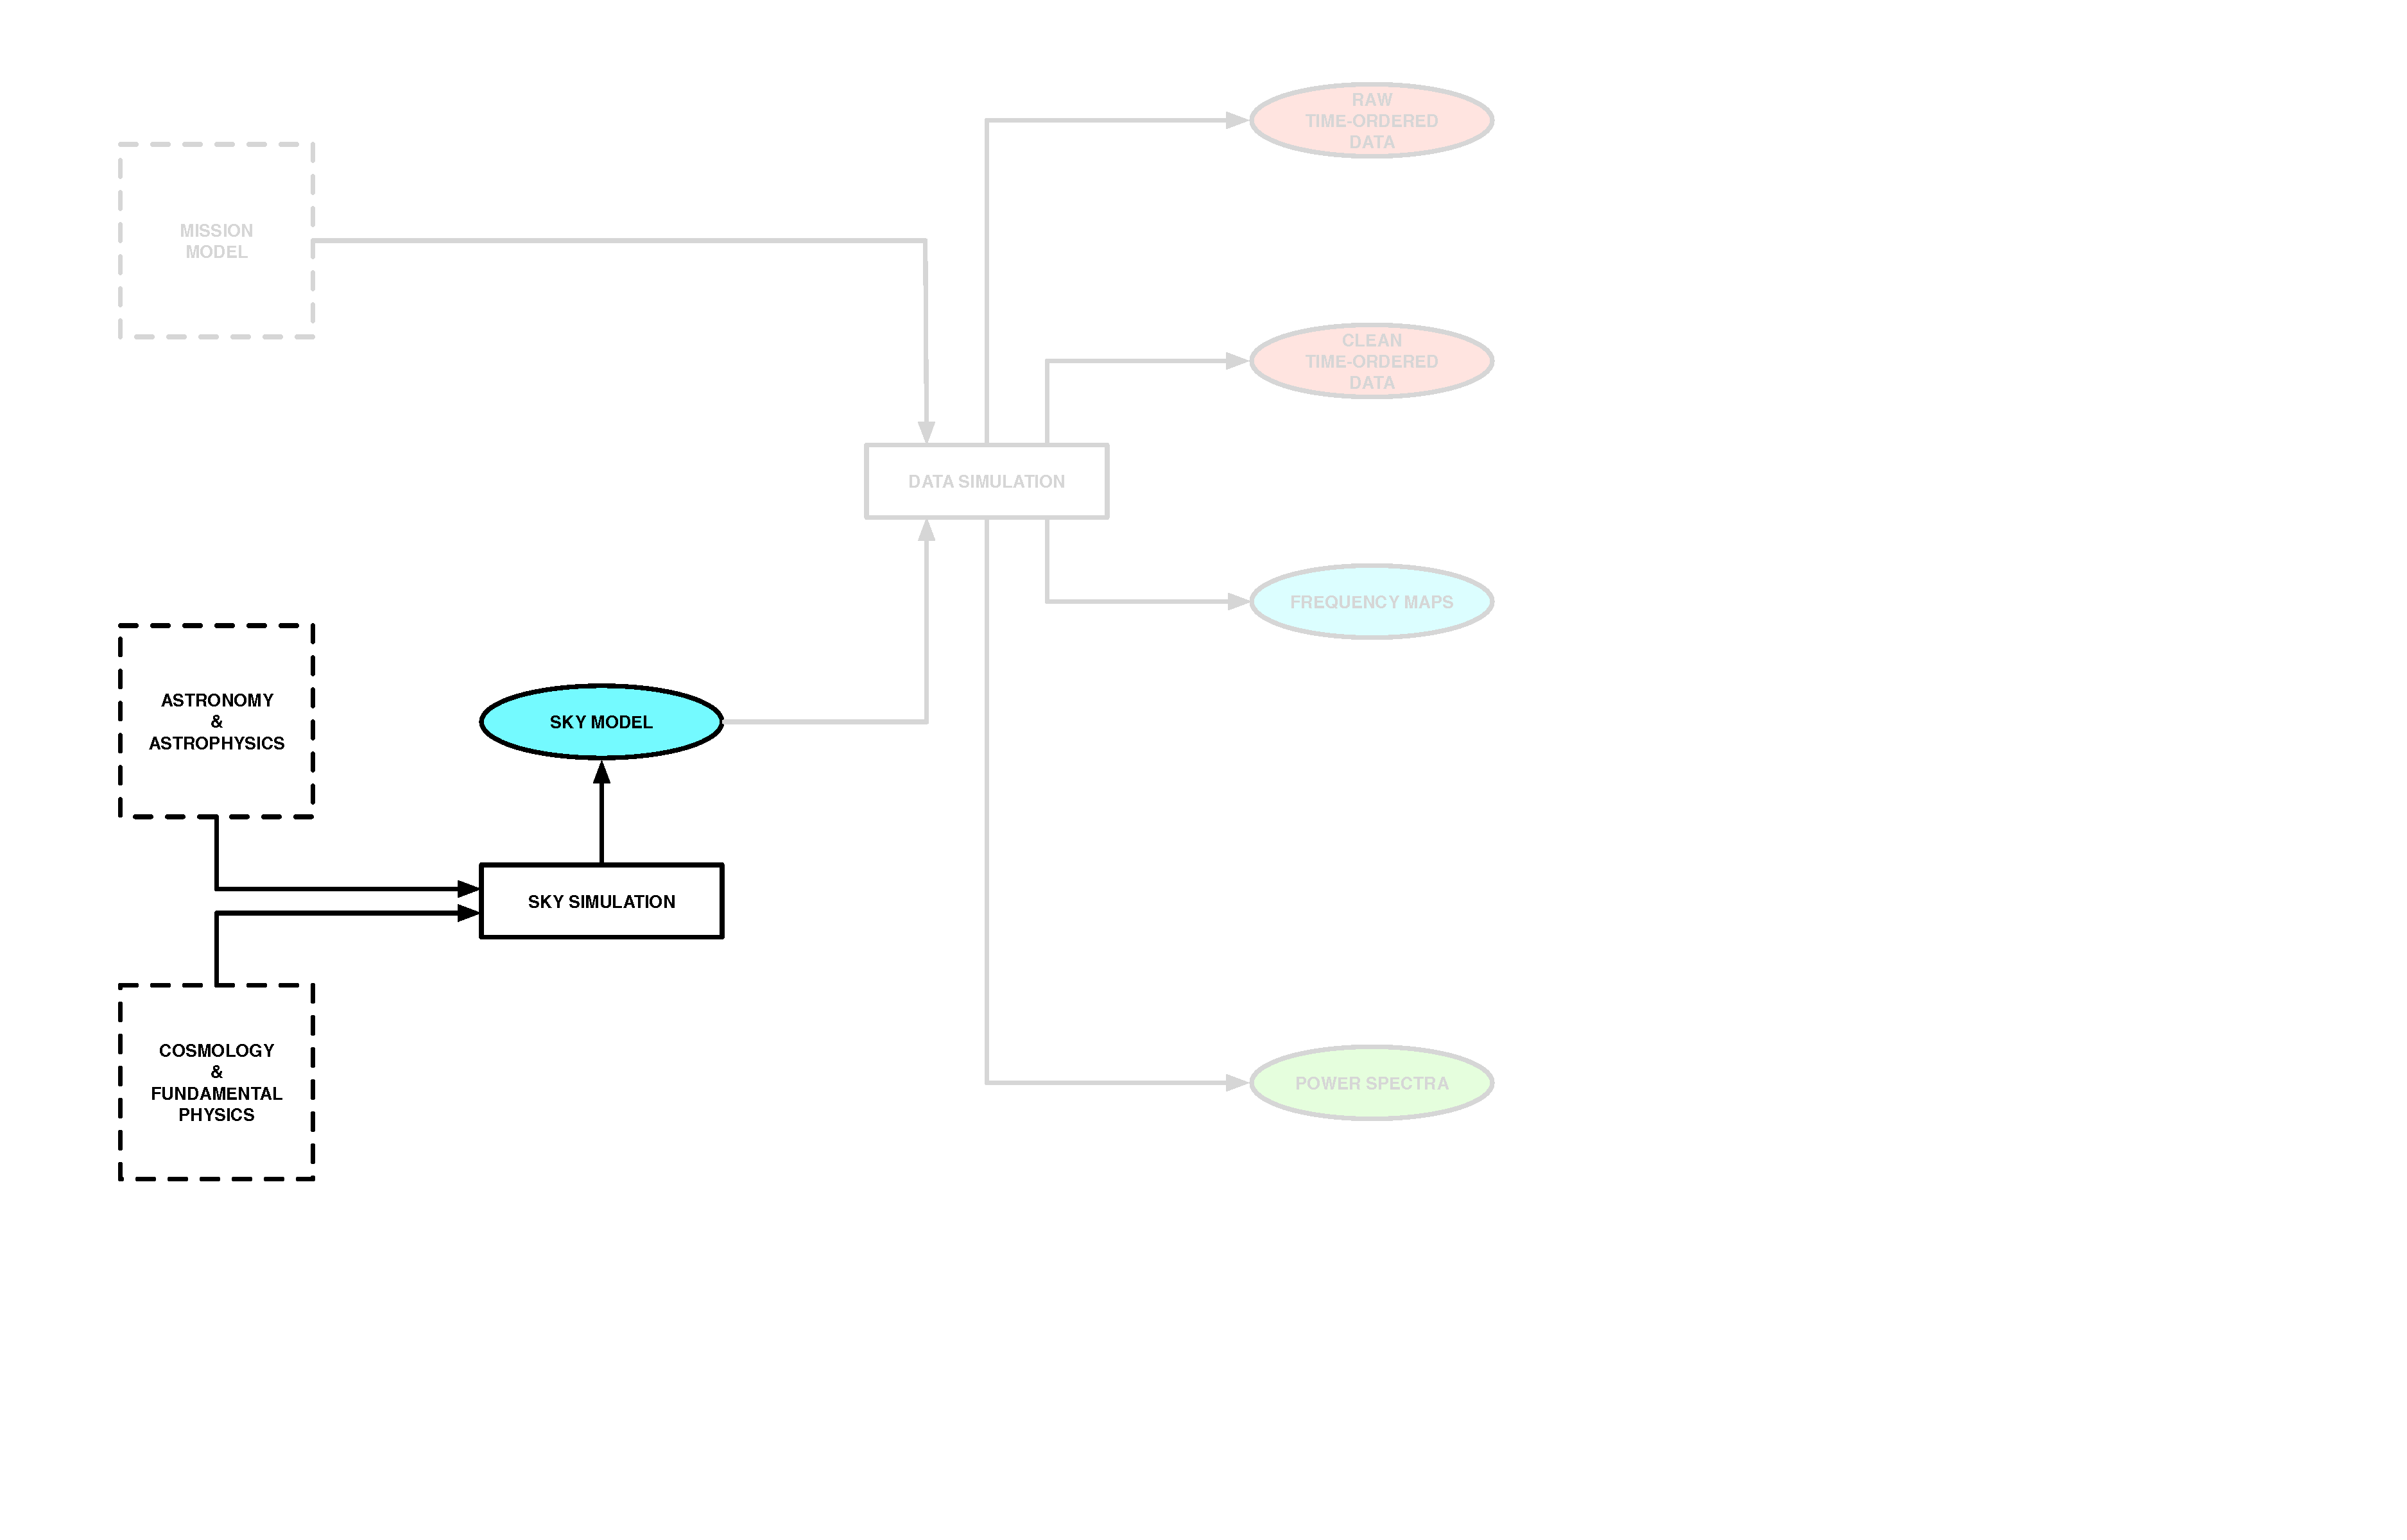
\includegraphics[width=1\textwidth]{Analysis/sm}
\caption{The sky modeling subset of the CMB simulation and data analysis pipeline}
\label{default}
\end{figure}

\subsection{CMB Secondary Anisotropies and Extragalactic Sources}

The key challenges for the extragalactic sky models of CMB-S4 are to provide fast and self-consistent simulations of CMB secondary anisotropies and extragalactic sources. These models will allow us to make more realistic forecasts. In our cosmological analyses they will allows us to Monte Carlo over the underlying astrophysical uncertainties of these secondaries and sources. Our plan to meet these challenges is modular and can be broken down as follows: 

\begin{itemize}
\item We will use full hydrodynamical simulations of cosmological volume as the basis to parametrically model the complicated {\it gastrophysical} processes associated with extragalactic foregrounds.
\item As the backbone of our model we will require fast simulations of growth of structure that generate halo catalogs for a large set of cosmological parameters.
\item To have self-consistent maps we will have a flexible pipeline that generates simulated all sky maps which applies the parametric models from the hydrodynamical simulations to our backbone large-scale structure simulations and halo catalogs.
\end{itemize}

Hydrodynamical simulations of cosmological volumes are currently available which we can already used to model extragalactic foregrounds. These simulations will be used for the development and testing phases of the simulation pipeline. However, they are limited in their size, sub-grid modeling accuracy, thus will not meet our accuracy requirements of CMB-S4. We will develop new full hydrodynamical simulations of cosmological volumes that include a variety of physical processes. An essential requirement of these simulations will be to capture growth and evolution of galaxies to clusters size halos throughout cosmic time at a sufficient spacial resolution. Hydrodynamic simulations of this size and scale are already computationally feasible, the challenges will be the appropriate modeling of radiative cooling, star formation, and feedback processes in order to capture the global stellar and gas contents of these halos.

There are many different approaches already developed to provide us with the underlying large-scale structure simulations that will we build our extragalactic model upon. They vary in speed which tend to inversely scale with accuracy. A benefit of our modular and flexible approach is that we do not need to limit ourselves to one approach. {\bf MORE}

Our final product will be all sky maps. They will be in HEALPIX format to seamlessly interface with galactic and CMB simulated maps.
{\bf MORE}

%\bibliography{cmbs4}

%%
%% Populate the .bib file with entries from SPIRES Bibtex (preferred)
%% or ADS Bibtex (if no SPIRES entry).
%%  SPIRES will also supply the CITATION line information; please include it.
%%


